\documentclass[../main.tex]{subfiles}

    \begin{document}

% Contents
\setcounter{page}{1}

%%%%%%%%%%%%%%
    % Introduction
    \clearpage

    \vspace*{\fill}
    \begin{center}
    \begin{minipage}{0.8\textwidth} % 80% de la largeur de la page (10% de marge de chaque côté)
        \justifying % Justifie
        \noindent
    \large{\textbf{\textcolor{UGEblue}{
Transports en commun, marche, vélo et micro-mobilité. Dix volets pour aménager des quartiers de gare du «~quart d'heure~» de la région Hauts-de-France, à l’échelle piétonnière et cyclable
    }}}
    \\\\
    \\
    \small{
Le regain d’intérêt pour \gras{le vélo} et l’émergence de \gras{la micro-mobilité} témoignent d’une transformation profonde des pratiques de mobilité quotidienne, portée par une demande croissante \gras{d’intermodalité}. La recherche menée met en relief le rôle clé de ces combinaisons modales diversifiées avec les réseaux de transport en commun, qui apparaissent comme une solution efficace aux défis \gras{des premiers et derniers kilomètres}.
    }
    \\\\
    \noindent
    \begin{tabular}{@{}m{0.25\textwidth} m{0.7\textwidth}@{}}
    \gras{\fontsize{40pt}{40pt}\selectfont
8~\%} & 
    \small{
C'est la part de voyageurs, parmi les usagers du réseau ferroviaire, ayant recours à un vélo ou un engin de déplacement pour se rabattre vers ou depuis une gare de la région.
    }
    \end{tabular}
    \\\\
    \small{
Nos estimations révèlent un potentiel de \gras{report modal} significatif de l’automobile vers ces pratiques intermodales. L’enjeu est double~: \gras{renforcer l’attractivité} des transports en commun tout en favorisant des déplacements de \gras{proximité} plus sobres. À cette fin, ces dix volets contribuent à articuler urbanisme et mobilité en promouvant une synergie entre le développement d’un véritable \gras{«~système vélo~»} et l’aménagement \gras{de territoires orientés vers les réseaux de transport en commun}.
    }
    \\\\
    \small{
Ce livrable vise à fournir \gras{aux décideurs, aménageurs et opérateurs de transport} des outils pour intégrer pleinement le vélo et la micro-mobilité dans les quartiers de gare. Ce \textsl{policy brief} formule ainsi \gras{dix recommandations stratégiques} pour créer des conditions favorables à la pratique intermodale et pour encourager un développement urbain à la fois orienté vers les transports en commun et soutenu par la marche, le vélo et la micro-mobilité.
    }

%%%%%%%%%%%%%%
    % Remerciements
    \vspace{0.25cm}
    \noindent\textcolor{lightgray}{\rule{\textwidth}{0.1pt}} % Line
    \vspace{0.25cm}
    \scriptsize{
    \textcolor{gray}{
    \begin{spacing}{0.8}
    \noindent{
Les auteurs adressent leurs sincères remerciements à \textbf{Kristel Hermel} pour son travail de facilitation graphique présenté ci-après, ainsi que pour sa relecture attentive dans le cadre de ses fonctions au sein de la Vice-Présidence à l'Appui aux Politiques Publiques et de la Vice-Présidence Recherche, où elle exerce également en tant que Présidente du comité qualité de l'Université Gustave Eiffel.
    }\end{spacing}
    }}
    

    \end{minipage}
    \end{center}
    \vspace*{\fill}

%%%%%%%%%%%%%%
    % Graphical abstract
    \newpage

\begin{center}\vspace*{10pt}
    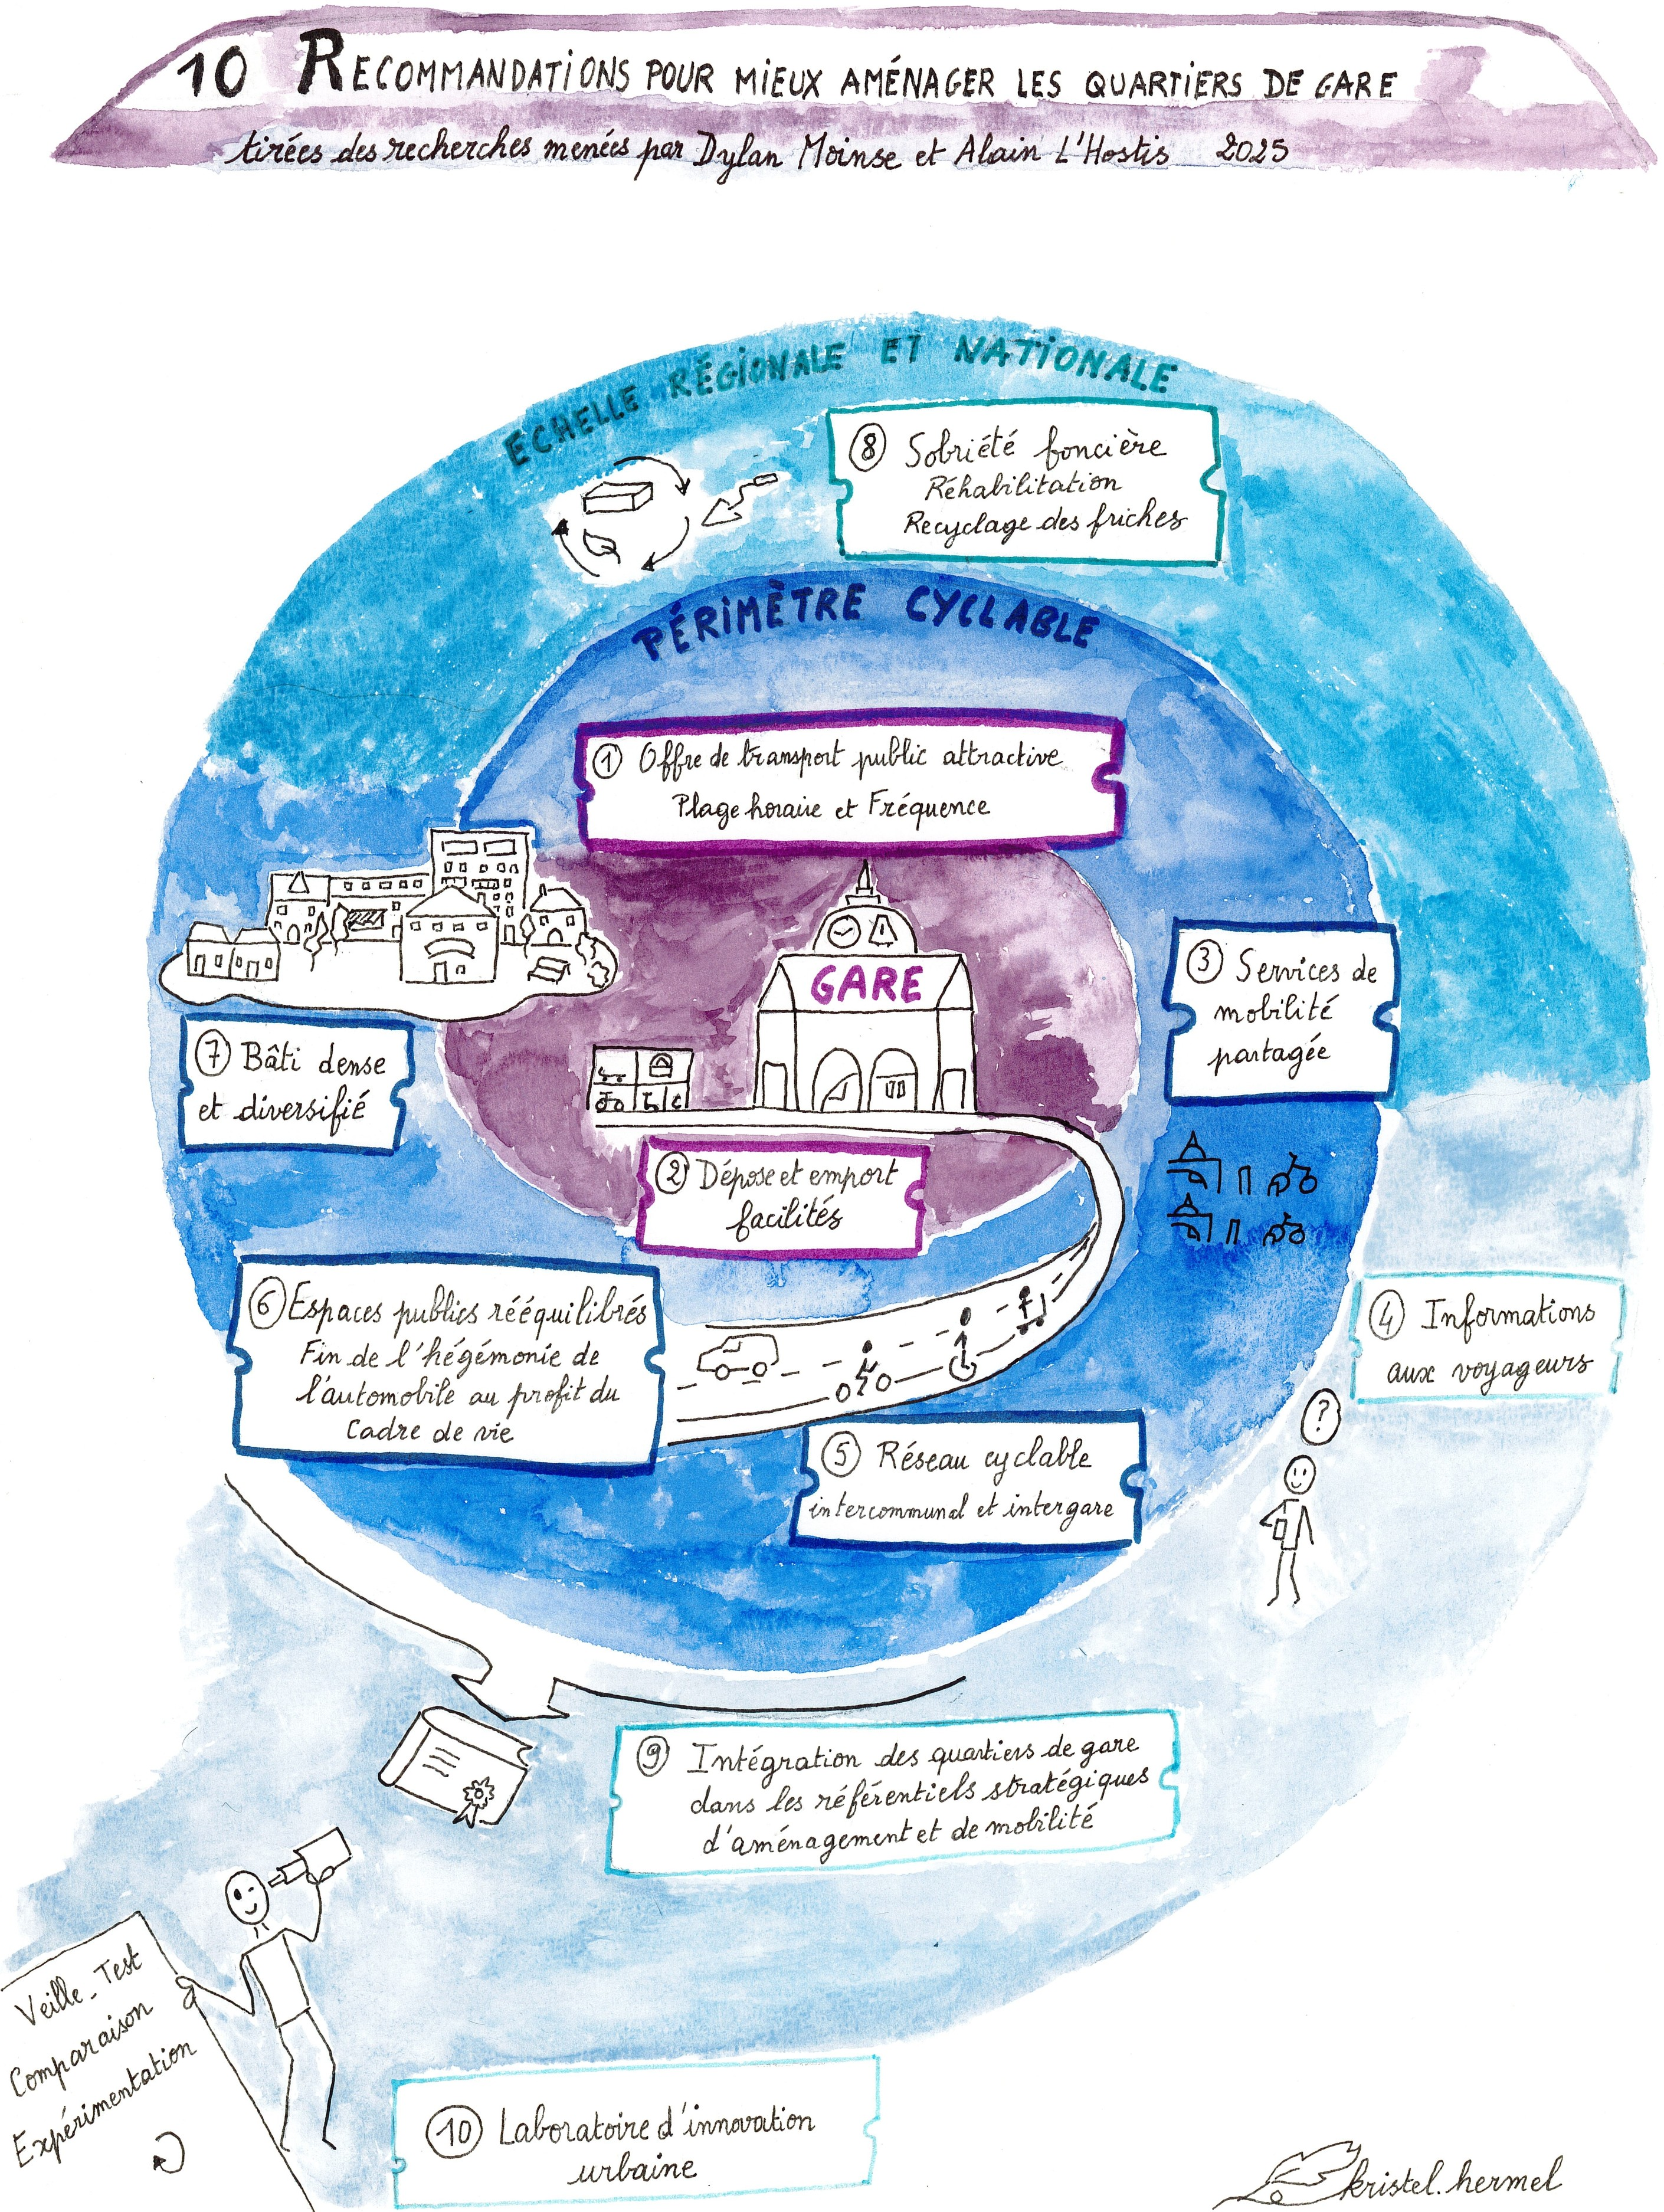
\includegraphics[width=0.95\columnwidth]{figures/policy-brief-graphical-abstract.jpg}
    \label{graphical-abstract}
    \vspace{0.3cm}
    \begin{flushright}
            \scriptsize{\textcolor{darkgray}{Autrice~: Kristel Hermel (2025)}}
    \end{flushright}
\end{center}
    \clearpage

    \end{document}